\documentclass{article}

\usepackage{amsmath}
\usepackage{amsfonts}
\usepackage{graphicx}
\usepackage{caption}
\usepackage{subcaption}
\usepackage{geometry}
 \geometry{
 a4paper,
 total={170mm,257mm},
 left=20mm,
 top=20mm,
 }
 
\author{Group 5}
\date{December 7, 2024}
\title{Conclusion Document}

\begin{document}
\maketitle

\section{Overview}

For the deep dive project, we choose to analyze the “Chicago Crime Dataset” with the primary objective of being able to predict future types of crime. As a secondary goal, we identify that if we are able to reasonably predict the types of crime, we can then perform evaluations such as feature importance to evaluate the importance and predictive power of the different features. This feature importance evaluation can be critical as an analysis tool in identifying predictive features, informing, and supporting the need for intervention in different communities or times. 

The rest of the conclusion document will briefly discuss motivations, key components in the model architecture, design, and finally some discussion on the findings.

\section{Motivation}

A successful and accurate predictive model has major decision making implications on the part of the police department. With an accurate predictive model, police departments can attempt to anticipate crime types at different locations. With extreme confidence in the model, this might translate to the police allocating resources in particular locations at different times of the day and year. Even without an extremely confident model, this can inform the need to provide different types of intervention such as informative interventions. That is, if the police department is aware that a particular type of crime spikes at a particular time of day or year, they can share important information that can aid in combating this crime. For example, informative posters on how to prevent burglaries, notifications of the dangers of walking home alone at a particular time of day, etc. 

\begin{figure}[h]
    \centering
    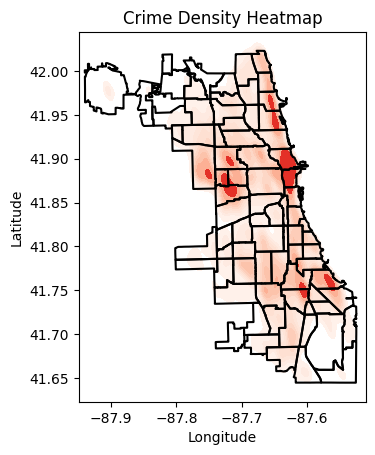
\includegraphics[width=0.5\linewidth]{deep-learning-im/crime-heatmap.png}
    \caption{Crime density heat-map overlaid on Chicago divided by county.}
    \label{fig:crime-heatmap}
\end{figure}

\section{Data Exploration}

By looking at the dataset through a data exploration, trends and commonalities arise to lead us to believe that a deep learning model will be able to learn something. There are a few aspects of the data that we explored: spatial and temporal. Within each of these, patterns and hot-spots even visible to the average person arises. In general, the analysis give the intuition that both spatial and temporal features are going to have a strong predictive power on future crime.

\begin{figure}
     \centering
     \begin{subfigure}[b]{0.45\textwidth}
         \centering
         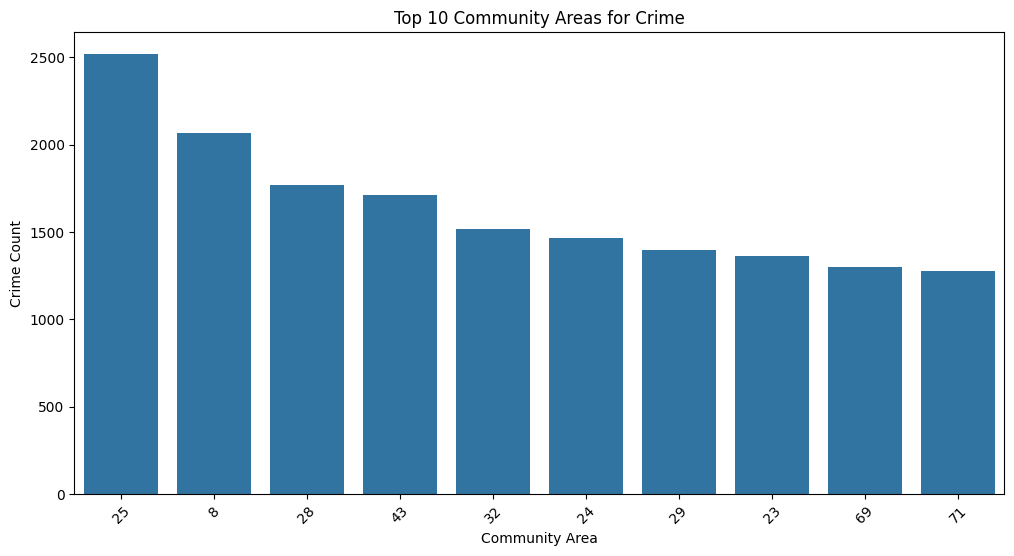
\includegraphics[width=\textwidth]{deep-learning-im/crime-community.png}
         \caption{Crime Count at Community Codes}
         \label{fig:crime-community}
     \end{subfigure}
     \hfill
     \begin{subfigure}[b]{0.45\textwidth}
         \centering
         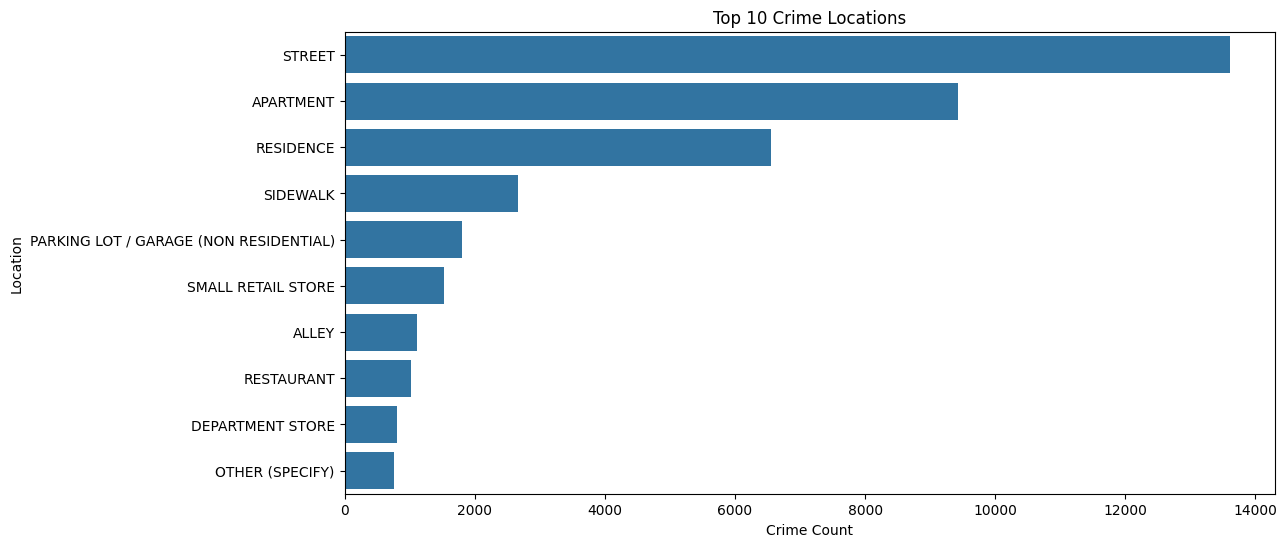
\includegraphics[width=\textwidth]{deep-learning-im/crime-location.png}
         \caption{Crime Count versus location}
         \label{fig:crime-location}
     \end{subfigure}
        \caption{Spatial Analysis of Crime}
        \label{fig:spatial}
\end{figure}


\subsection{Spatial.} We begin our discussion by discussing and showing the crime density heat map overlaid the city and suburbs of Chicago in Fig. \ref{fig:crime-heatmap}. Through this figure, we can see four major regions whose crime dominates the frequency of crime in the region. Fig. \ref{fig:spatial} shows the crime counts measured against spatial values such as the community code and the location. These graphs demonstrate that there are clear relationships between the location and the crime. 

\subsection{Temporal.} Fig. \ref{fig:temporal} demonstrate clear trends in the temporal information. This provides the intuition that the temporal values are going to have predictive power. In particular, the crime by the month and crime by time of day demonstrate the most predictive power. We see both that during the winter months, crime tends to fall. As the weather heats up, the crime rate increases. Crime by time of day seems to be pretty stead with the exception of the evening. Crime in the evening is by far the most common time for crime.

\begin{figure}
     \centering
     \begin{subfigure}[b]{0.3\textwidth}
         \centering
         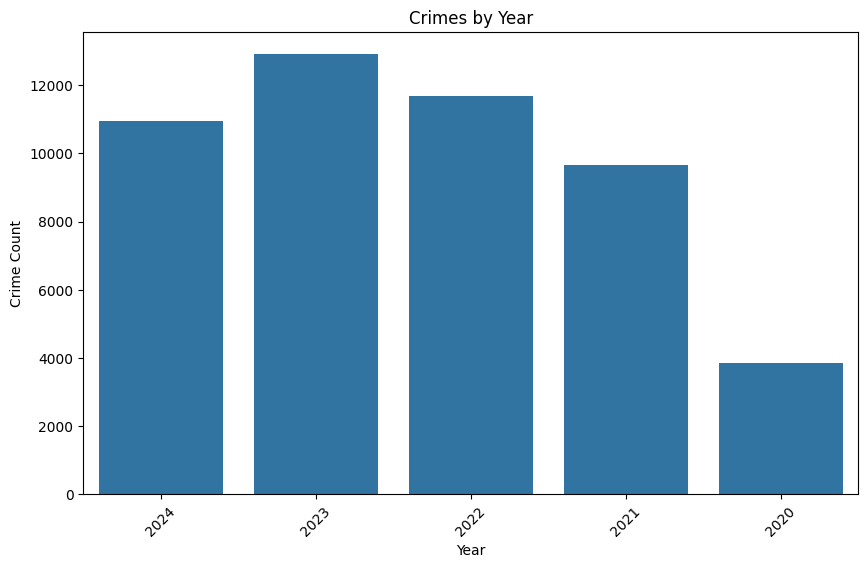
\includegraphics[width=\textwidth]{deep-learning-im/crime-year.png}
         \caption{Crime by Year}
         \label{fig:crime-community}
     \end{subfigure}
     \hfill
     \begin{subfigure}[b]{0.3\textwidth}
         \centering
         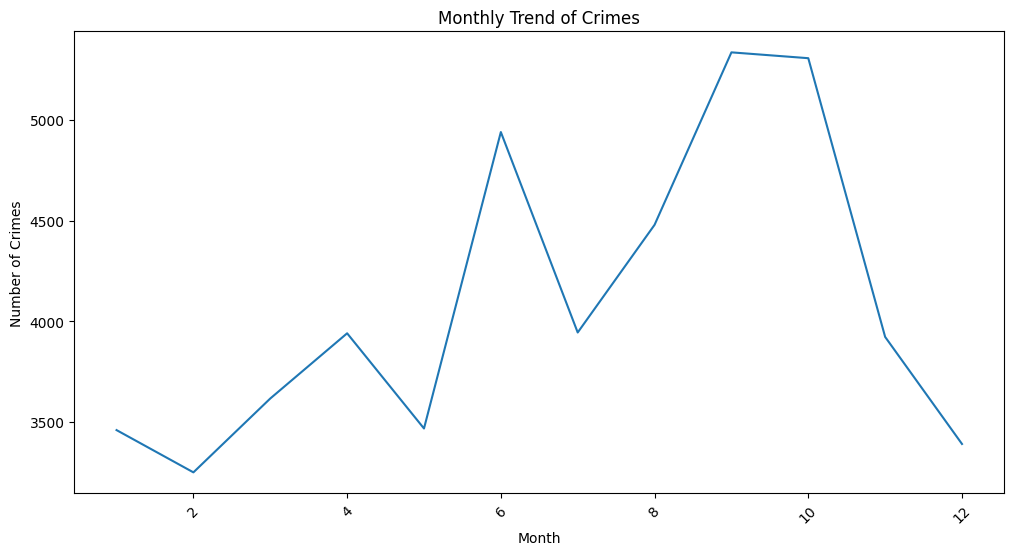
\includegraphics[width=\textwidth]{deep-learning-im/crime-month.png}
         \caption{Crime by Months}
         \label{fig:crime-location}
     \end{subfigure}
     \begin{subfigure}[b]{0.3\textwidth}
         \centering
         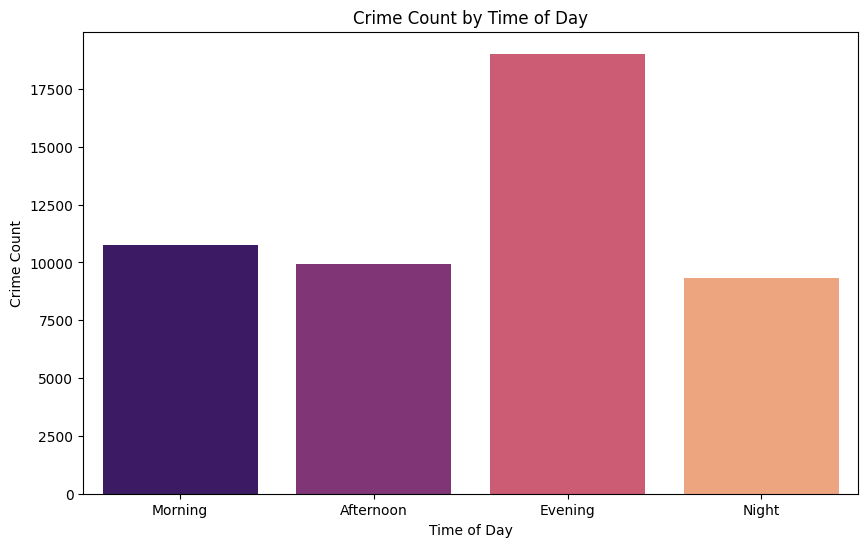
\includegraphics[width=\textwidth]{deep-learning-im/crime-time.png}
         \caption{Crime by Time}
         \label{fig:crime-location}
     \end{subfigure}
        \caption{Temporal Graphs of Crime}
        \label{fig:temporal}
\end{figure}

\section{Model}
In this section, we briefly discuss some key aspects of the model and technical challenges encountered. 

\subsection{Temporal Patterns Matter}
The LSTM layer successfully records crime trends across time, demonstrating that crimes might follow predictable patterns according to the time of day or night, such as increased activity on weekends or at night.

\subsection{Robustness Against Noise}
The model's capacity to generalize is enhanced by dropout and batch normalization, underscoring the significance of managing unpredictability in actual crime data, such as irregularities in location reporting.

\subsection{Efficiency in Decision-Making}
The Adam optimizer guarantees faster learning, allowing for quicker insights into crime categories. This is essential for prompt actions in urban safety planning.

\subsection{Feature Transformations are Key}
By embedding category characteristics like "crime type" and normalizing geographical coordinates, the model is able to identify subtle contextual and spatial correlations, including recurring hotspots for particular crimes.

\subsection{Scalability for Urban Analysis}
The model's modular architecture allows it to be tailored to various cities or bigger datasets, opening the door for more extensive uses in predictive policing and urban safety.

\subsection{Categorical Prediction}
One challenge that we did not expect from the beginning was the categorical nature of crime type. As we have seen in class, performing prediction on categorical data is not simple. Even in the regression case, we see that we introduce an entirely new formatting of data, loss function, and analysis. In the deep learning setting, we encountered that the models that we discussed in class would not work out of the box and would require modifications. Albeit, there are resources for performing categorical predictions for the most popular deep models, but this required further research than we expected. 

\section{Results}

\subsection{Feature Importance}

\subsection{Performance}

% Comparison to baseline 


\end{document}